\documentclass{VUMIFPSkursinis}
\usepackage{algorithmicx}
\usepackage{algorithm}
\usepackage{algpseudocode}
\usepackage{amsfonts}
\usepackage{amsmath}
\usepackage{bm}
\usepackage{caption}
\usepackage{color}
\usepackage{float}
\usepackage{graphicx}
\usepackage{listings}
\usepackage{subfig}
\usepackage{wrapfig}
\usepackage{sectsty}
\usepackage{enumerate}
\usepackage{longtable}
\usepackage[export]{adjustbox}
\usepackage{rotating}
\usepackage{hhline}
\usepackage{multirow}
\usepackage{tabularx}
\usepackage{array}
\usepackage{booktabs,calc}
\usepackage{tabularx,colortbl}
\usepackage[table]{xcolor}  
\usepackage{longtable}  

\usepackage{enumitem}
%PAKEISTA, tarpai tarp sąrašo elementų
\setitemize{noitemsep,topsep=0pt,parsep=0pt,partopsep=0pt}
\setenumerate{noitemsep,topsep=0pt,parsep=0pt,partopsep=0pt}
\allsectionsfont{\centering}
% Titulinio aprašas
\university{Vilniaus universitetas}
\faculty{Matematikos ir informatikos fakultetas}
\department{Programų sistemų katedra}
\papertype{Programų sistemų inžinerijos I laboratorinis darbas}
\title{Internetinis aukcionas}
\titleineng{Digital Auction}
\status{2 kurso 4 grupės studentai}
\author{Andrejus Voitovas}
\secondauthor{Eglė Puodžiūnaitė}
\thirdauthor{Kasparas Kralikas}
\fourthauthor{Ieva Vizgirdaitė} % Pridėti antrą autorių
\supervisor{asist. dr. Vytautas Valaitis}
\date{Vilnius – \the\year}

% Nustatymai
% \setmainfont{Palemonas}   % Pakeisti teksto šriftą į Palemonas (turi būti įdiegtas sistemoje)
\bibliography{bibliografija}

\begin{document}
% PAKEISTA
\maketitle
\cleardoublepage\pagenumbering{arabic}
\setcounter{page}{2}
\sectionnonum{ANOTACIJA}
Šiame dokumente sistema analizuojama taikant ICONIX metodą. Pateikiami funkciniai ir nefunkciniai reikalavimai, apibrėžiamas struktūrinis dalykinės srities modelis. Taip pat aprašomos sistemoje atliekamos užduotys, analizuojami pagrindiniai ir alternatyvūs užduočių scenarijai. Rašant šį dokumentą buvo naudojamasi:
\\1. dr. Vytauto Valaičio internetiniu puslapiu (https://klevas.mif.vu.lt/~valaitis/)
\\2. doc., dr. Karolio Petrausko internetiniu puslapiu (http://klevas.mif.vu.lt/~karolis/)
\\3. Latex programa
\\4. lab. asst. Jono Brusoko parengtais kursinio darbo šablonais (https://gitlab.com/JohnLogic/SE-course-work-template)
\newpage
%TURINYS
\tableofcontents

\sectionnonum{ĮVADAS}
Internetinis aukcionas kuriamas siekiant išplėsti dalyvavimą aukcionuose nuotoliniu
būdu. Tinklalapis suteikia galimybę klientams paprastai ir patogiai dalyvauti aukcionuose bet kuriuo paros metu. Dokumente pateikiamas pagrindinis programos funkcionalumas ir tam tikri ribojimai jos kūrimui. Pasitelkiant ICONIX metodą sudaromi užduočių scenarijai, apibrėžiamos pagrindinės kuriamos sistemos esybės, sudaromas struktūrinis dalykinės srities modelis. Šis dokumentas padeda toliau projektuoti ir nuspręsti, kaip sistema turėtų būti įgyvendinta.
\\\textbf{Dalykinė sritis}
\\Internetinis aukcionas.
\\\textbf{Probleminė sritis} 
\\Internetinis aukcionas suteiktų galimybę greitai ir paprastai dalyvauti aukcionuose.
\\\textbf{Darbo pagrindas}
\\Dokumentas parengtas kaip Programų sistemų inžinerijos II dalies I laboratorinis darbas.
\\\textbf{Darbo užduotys}
\\1. Suformuluoti funkcinius reikalavimus.
\\2. Suformuluoti nefunkcinius reikalavimus.
\\3. Apibrėžti struktūrinį dalykinės srities modelį.
\\4. Aprašyti sistemoje atliekamas užduotis.
\newpage
\section{FUNKCINIAI REIKALAVIMAI}
Šiame skyriuje pateikiami funkciniai reikalavimai – nagrinėjami scenarijai, ką sistema turi daryti, kaip elgtis vienu ar kitu atveju.

\subsection{Internetinės svetainės langai}
\begin{table}[H]
	\caption{Funkciniai reikalavimai. Internetinės svetainės langai.}
	\begin{tabular}{|p{1cm}|p{1cm}|p{11,5cm}|p{3,5cm}|}
		\hline 
		\rowcolor{gray!50}
		\multicolumn{2}{|c|}{{\bfseries Kodas}}&
		\multicolumn{1}{c|}{{\bfseries Reikalavimas}}&
		\multicolumn{1}{c|}{{\bfseries Svarba}}\\
		\hline
		\rowcolor{lightgray}
		\multicolumn{4}{|c|}{Internetinės svetainės langai}\\		
		
		\hline
		\multicolumn{2}{|c|}{FR 1.1}&
		{Svetainės langai „Registracija“, „Prisijungimas“, „Pagrindinis puslapis“, „Taisyklės“ turi būti matomi visiems naudotojams.
		}&		
		\multicolumn{1}{c|}{Būtina}\\
		\hline
		\multicolumn{1}{|c}{}&
		\multicolumn{1}{c|}{FR 1.2}&
		{Svetainės langai „Mano profilis“, „Prekės įkėlimas“, „Prekės aukcionas“ turi būti matomi visiems prisijungusiems naudotojams.
		}&		
		\multicolumn{1}{c|}{Būtina}\\
		\hline
		\multicolumn{1}{|c}{}&
		\multicolumn{1}{c|}{FR 1.3}&
		{Svetainės langai „Visi aukcionai“, „Naudotojai“  turi būti matomas sistemos adminstratoriams.
		}&
		\multicolumn{1}{c|}{Būtina}\\	
		\hline		
	\end{tabular}		
\end{table}

\subsection{Registracija}
\begin{table}[H]
	\caption{Funkciniai reikalavimai. Registracija.}
	\begin{tabular}{|p{1cm}|p{1cm}|p{11,5cm}|p{3,5cm}|}
		\hline 
		\rowcolor{gray!50}
		\multicolumn{2}{|c|}{{\bfseries Kodas}}&
		\multicolumn{1}{c|}{{\bfseries Reikalavimas}}&
		\multicolumn{1}{c|}{{\bfseries Svarba}}\\
		\hline
		\rowcolor{lightgray}
		\multicolumn{4}{|c|}{Registracija}\\		
		
		\hline
		\multicolumn{2}{|c|}{FR 2.1}&
		{Naudotojui suvedus visą reikiamą informaciją ir nuspaudus mygtuką registruotis, jis turi būti priregistruojamas internetinėje sveitainėje.
		}&		
		\multicolumn{1}{c|}{Būtina}\\
		\hline
		\multicolumn{1}{|c}{}&
		\multicolumn{1}{c|}{FR 2.2}&
		{Naudotojui nesuvedus informacijos į visus privalomus laukus jis neturi būti priregistruojamas sistemoje bei registracijos puslapyje turi būti išmetamas klaidos pranešimas, pranešantis, jog reikia užpildyti visus privalomus laukus.
		}&		
		\multicolumn{1}{c|}{Būtina}\\
		\hline	
		\multicolumn{1}{|c}{}&
		\multicolumn{1}{c|}{FR 2.3}&
		{Registruojantis naudotojas turi įvesti internetinėje svetainėje dar nepriregistruotą el. pašto adresą.
		}&
		\multicolumn{1}{c|}{Būtina}\\									
		\hline
	\end{tabular}		
\end{table}

\subsection{Prisijungimas}
\begin{table}[H]
	\caption{Funkciniai reikalavimai. Prisijungimas.}
	\begin{tabular}{|p{1cm}|p{1cm}|p{11,5cm}|p{3,5cm}|}
		\hline 
		\rowcolor{gray!50}
		\multicolumn{2}{|c|}{{\bfseries Kodas}}&
		\multicolumn{1}{c|}{{\bfseries Reikalavimas}}&
		\multicolumn{1}{c|}{{\bfseries Svarba}}\\
		\hline
		\rowcolor{lightgray}
		\multicolumn{4}{|c|}{Prisijungimas}\\		
		
		\hline
		\multicolumn{2}{|c|}{FR 3.1}&
		{Naudotojui suvedus tinkamus prisijungimo duomenis jis turi būti prijungiamas prie sistemos.
		}&		
		\multicolumn{1}{c|}{Būtina}\\
		\hline
		\multicolumn{1}{|c}{}&
		\multicolumn{1}{c|}{FR 3.2}&
		{Naudotojui netinkamai įvedus prisijungimo duomenis jis neturi būti prijungiamas prie sistemos bei turi būti išmetamas klaidos pranešimas.
		}&		
		\multicolumn{1}{c|}{Būtina}\\
		\hline	
		\multicolumn{1}{|c}{}&
		\multicolumn{1}{c|}{FR 3.3}&
		{Naudotojo bandymų prisijungti prie sistemos skaičius neturi būti ribojamas.
		}&
		\multicolumn{1}{c|}{Būtina}\\									
		\hline
	\end{tabular}		
\end{table}

\subsection{Atsijungimas}

\begin{table}[H]
	\caption{Funkciniai reikalavimai. Atsijungimas.}
	\begin{tabular}{|p{1cm}|p{1cm}|p{11,5cm}|p{3,5cm}|}
		\hline 
		\rowcolor{gray!50}
		\multicolumn{2}{|c|}{{\bfseries Kodas}}&
		\multicolumn{1}{c|}{{\bfseries Reikalavimas}}&
		\multicolumn{1}{c|}{{\bfseries Svarba}}\\
		\hline
		\rowcolor{lightgray}
		\multicolumn{4}{|c|}{Atsijungimas}\\		
		
		\hline
		\multicolumn{2}{|c|}{FR 4.1}&
		{Naudotojas paspaudęs mygtuką atsijungti turi būti atjungiamas nuo sistemos.
		}&		
		\multicolumn{1}{c|}{Būtina}\\
		\hline
	\end{tabular}		
\end{table}

\subsection{Paskyros valdymas}

\begin{table}[H]
	\caption{Funkciniai reikalavimai. Paskyros valdymas.}
	\begin{tabular}{|p{1cm}|p{1cm}|p{11,5cm}|p{3,5cm}|}
		\hline 
		\rowcolor{gray!50}
		\multicolumn{2}{|c|}{{\bfseries Kodas}}&
		\multicolumn{1}{c|}{{\bfseries Reikalavimas}}&
		\multicolumn{1}{c|}{{\bfseries Svarba}}\\
		\hline
		\rowcolor{lightgray}
		\multicolumn{4}{|c|}{Paskyros valdymas}\\				
		\hline
		\multicolumn{2}{|c|}{FR 5.1}&
		{Naudotojui paspaudus mygtuką „Mano profilis“ turi būti matoma visa žinoma informacija apie naudotoją.
		}&		
		\multicolumn{1}{c|}{Būtina}\\
		\hline
		\multicolumn{1}{|c}{}&
		\multicolumn{1}{c|}{FR 5.2}&
		{Naudotojui paspaudus mygtuką „Pakeisti slaptažodį“, įvedus tinkamą seną ir naują slaptažodžius bei paspaudus mygtuką „Patvirtinti“ slaptažodis turi būti pakeičiamas į naują.
		}&		
		\multicolumn{1}{c|}{Būtina}\\
		\hline
		\multicolumn{1}{|c}{}&
		\multicolumn{1}{c|}{FR 5.3}&
		{Naudotojui paspaudus mygtuką „Pakeisti slaptažodį“ ir įvedus netinkamą seną slaptažodį turi būti išvedamas klaidos pranešimas.
		}&
		\multicolumn{1}{c|}{Būtina}\\	
		\hline		
	\end{tabular}		
\end{table}

\subsection{Taisyklės}
\begin{table}[H]
	\caption{Funkciniai reikalavimai. Taisyklės}
	\begin{tabular}{|p{1cm}|p{1cm}|p{11,5cm}|p{3,5cm}|}
		\hline 
		\rowcolor{gray!50}
		\multicolumn{2}{|c|}{{\bfseries Kodas}}&
		\multicolumn{1}{c|}{{\bfseries Reikalavimas}}&
		\multicolumn{1}{c|}{{\bfseries Svarba}}\\
		\hline
		\rowcolor{lightgray}
		\multicolumn{4}{|c|}{Taisyklės}\\		
		
		\hline
		\multicolumn{2}{|c|}{FR 6.1}&
		{Taisyklės turi būti matomos puslapyje „Taisyklės“.
		}&		
		\multicolumn{1}{c|}{Būtina}\\
		\hline
		\multicolumn{1}{|c}{}&
		\multicolumn{1}{c|}{FR 6.2}&
		{Visas taisyklių sąrašas turi būti pateikiamas viename puslapyje.
		}&		
		\multicolumn{1}{c|}{Būtina}\\
		\hline	
		\multicolumn{1}{|c}{}&
		\multicolumn{1}{c|}{FR 6.3}&
		{Taisyklės turi būti matomos visiems sistemos naudotojams.
		}&
		\multicolumn{1}{c|}{Būtina}\\									
		\hline
	\end{tabular}		
\end{table}

\subsection{Pagrindinis puslapis}
\begin{table}[H]
	\caption{Funkciniai reikalavimai. Pagrindinis puslapis}
	\begin{tabular}{|p{1cm}|p{1cm}|p{11,5cm}|p{3,5cm}|}
		\hline 
		\rowcolor{gray!50}
		\multicolumn{2}{|c|}{{\bfseries Kodas}}&
		\multicolumn{1}{c|}{{\bfseries Reikalavimas}}&
		\multicolumn{1}{c|}{{\bfseries Svarba}}\\
		\hline
		\rowcolor{lightgray}
		\multicolumn{4}{|c|}{Pagrindinis puslapis}\\		
		
		\hline
		\multicolumn{2}{|c|}{FR 7.1}&
		{Aktyvūs aukcionai turi būti matomi puslapyje „Pagrindinis puslapis“.
		}&		
		\multicolumn{1}{c|}{Būtina}\\
		\hline
		\multicolumn{1}{|c}{}&
		\multicolumn{1}{c|}{FR 7.2}&
		{Visas aktyvių aukcionų sąrašas turi būti pateikiamas viename puslapyje.
		}&		
		\multicolumn{1}{c|}{Būtina}\\
		\hline	
		\multicolumn{1}{|c}{}&
		\multicolumn{1}{c|}{FR 7.3}&
		{Pagrindinis puslapis turi būti matomas visiems sistemos naudotojams.
		}&
		\multicolumn{1}{c|}{Būtina}\\									
		\hline
		\multicolumn{1}{|c}{}&
		\multicolumn{1}{c|}{FR 7.4}&
		{Prisijungusiam naudotojui paspaudus ant aktyvaus aukciono mygtuko „Daugiau informacijos“ turi būti atidaromas puslapis „Prekės aukcionas“.
		}&
		\multicolumn{1}{c|}{Būtina}\\									
		\hline
	\end{tabular}		
\end{table}

\subsection{Prekės įkėlimas}
\begin{table}[H]
	\caption{Funkciniai reikalavimai. Prekės įkėlimas}
	\begin{tabular}{|p{1cm}|p{1cm}|p{11,5cm}|p{3,5cm}|}
		\hline 
		\rowcolor{gray!50}
		\multicolumn{2}{|c|}{{\bfseries Kodas}}&
		\multicolumn{1}{c|}{{\bfseries Reikalavimas}}&
		\multicolumn{1}{c|}{{\bfseries Svarba}}\\
		\hline
		\rowcolor{lightgray}
		\multicolumn{4}{|c|}{Prekės įkėlimas}\\		
		
		\hline
		\multicolumn{2}{|c|}{FR 8.1}&
		{Puslapis „Prekės įkėlimas“ turi būti matomas visiems prijungusiems naudotojams.
		}&		
		\multicolumn{1}{c|}{Būtina}\\
		\hline
		\multicolumn{1}{|c}{}&
		\multicolumn{1}{c|}{FR 8.2}&
		{Naudotojui suvedus visą reikiamą informaciją apie aukciono prekę bei paspaudus mygtuką „Patvirtinti“ turi būti sukuriamas aukcionas.
		}&		
		\multicolumn{1}{c|}{Būtina}\\
		\hline	
		\multicolumn{1}{|c}{}&
		\multicolumn{1}{c|}{FR 8.3}&
		{Naudotojui nesuvedus informacijos į visus privalomus laukus aukcionas neturi būti sukuriamas bei prekės įkėlimo puslapyje turi būti išmetamas klaidos pranešimas, pranešantis, jog reikia užpildyti visus privalomus laukus.
		}&
		\multicolumn{1}{c|}{Būtina}\\									
		\hline
	\end{tabular}		
\end{table}

\subsection{Prekės aukcionas}
\begin{table}[H]
	\caption{Funkciniai reikalavimai. Prekės aukcionas}
	\begin{tabular}{|p{1cm}|p{1cm}|p{11,5cm}|p{3,5cm}|}
		\hline 
		\rowcolor{gray!50}
		\multicolumn{2}{|c|}{{\bfseries Kodas}}&
		\multicolumn{1}{c|}{{\bfseries Reikalavimas}}&
		\multicolumn{1}{c|}{{\bfseries Svarba}}\\
		\hline
		\rowcolor{lightgray}
		\multicolumn{4}{|c|}{Prekės aukcionas}\\				
		\hline
		\multicolumn{2}{|c|}{FR 9.1}&
		{Puslapis „Prekės aukcionas“ turi būti matomas visiems prijungusiems naudotojams.
		}&		
		\multicolumn{1}{c|}{Būtina}\\
		\hline
		\multicolumn{1}{|c}{}&
		\multicolumn{1}{c|}{FR 9.2}&
		{Puslapyje „Prekės aukcionas“ aukcionas yra aktyvus tokį laikotarpį, kokį nurodė naudotojas sukūręs aukcioną.
		}&		
		\multicolumn{1}{c|}{Būtina}\\
		\hline	
		\multicolumn{1}{|c}{}&
		\multicolumn{1}{c|}{FR 9.3}&
		{Jei aukciono statusas yra „Aktyvus“ naudotojai gali siūlyti savo kainas jas įvedus į kainos laukelį ir paspaudus mygtuką „Patvirtinti“.
		}&
		\multicolumn{1}{c|}{Būtina}\\									
		\hline
		\multicolumn{1}{|c}{}&
		\multicolumn{1}{c|}{FR 9.4}&
		{Naudotojo siūloma kaina negali būti mažesnė už jau pasiūlytą kainą. Jei naudotojas bando pasiūlyti mažesnę kainą, turi būti išmetamas klaidos pranešimas, jog kaina yra per maža.
		}&
		\multicolumn{1}{c|}{Būtina}\\									
		\hline
		\multicolumn{1}{|c}{}&
		\multicolumn{1}{c|}{FR 9.5}&
		{Praėjus naudotojo nurodytam aukciono laikotarpiui jo statusas turi automatiškai pasikeisti į „Pasibaigęs“, puslapyje „Prekės aukcionas“ turi būti parašytas aukciono laimėtojas, o kainos siūlymo laukelis nebeturi būti matomas.
		}&
		\multicolumn{1}{c|}{Būtina}\\									
		\hline
	\end{tabular}		
\end{table}

\subsection{Visi aukcionai}
\begin{table}[H]
	\caption{Funkciniai reikalavimai. Visi aukcionai}
	\begin{tabular}{|p{1cm}|p{1cm}|p{11,5cm}|p{3,5cm}|}
		\hline 
		\rowcolor{gray!50}
		\multicolumn{2}{|c|}{{\bfseries Kodas}}&
		\multicolumn{1}{c|}{{\bfseries Reikalavimas}}&
		\multicolumn{1}{c|}{{\bfseries Svarba}}\\
		\hline
		\rowcolor{lightgray}
		\multicolumn{4}{|c|}{Visi aukcionai}\\				
		\hline
		\multicolumn{2}{|c|}{FR 10.1}&
		{Puslapis „Visi aukcionai“ turi būti matomas tik sistemos administratoriams.
		}&		
		\multicolumn{1}{c|}{Būtina}\\
		\hline
		\multicolumn{1}{|c}{}&
		\multicolumn{1}{c|}{FR 10.2}&
		{Puslapyje „Visi aukcionai“ turi būti matomas visų aktyvių ir pasibaigusių aukcionų sąrašas.
		}&		
		\multicolumn{1}{c|}{Būtina}\\
		\hline	
		\multicolumn{1}{|c}{}&
		\multicolumn{1}{c|}{FR 10.3}&
		{Visas aukcionų sąrašas turi būti pateikiamas viename puslapyje.
		}&
		\multicolumn{1}{c|}{Būtina}\\									
		\hline
		\multicolumn{1}{|c}{}&
		\multicolumn{1}{c|}{FR 10.4}&
		{Puslapyje administratorius turi turėti galimybę ištrinti aukcioną.
		}&
		\multicolumn{1}{c|}{Būtina}\\									
		\hline
	\end{tabular}		
\end{table}

\subsection{Naudotojai}
\begin{table}[H]
	\caption{Funkciniai reikalavimai. Naudotojai}
	\begin{tabular}{|p{1cm}|p{1cm}|p{11,5cm}|p{3,5cm}|}
		\hline 
		\rowcolor{gray!50}
		\multicolumn{2}{|c|}{{\bfseries Kodas}}&
		\multicolumn{1}{c|}{{\bfseries Reikalavimas}}&
		\multicolumn{1}{c|}{{\bfseries Svarba}}\\
		\hline
		\rowcolor{lightgray}
		\multicolumn{4}{|c|}{Naudotojai}\\				
		\hline
		\multicolumn{2}{|c|}{FR 11.1}&
		{Puslapis „Naudotojai“ turi būti matomas tik sistemos administratoriams.
		}&		
		\multicolumn{1}{c|}{Būtina}\\
		\hline
		\multicolumn{1}{|c}{}&
		\multicolumn{1}{c|}{FR 11.2}&
		{Puslapyje „Naudotojai“ turi būti matomas visų naudotojų sąrašas.
		}&		
		\multicolumn{1}{c|}{Būtina}\\
		\hline	
		\multicolumn{1}{|c}{}&
		\multicolumn{1}{c|}{FR 11.3}&
		{Visas naudotojų sąrašas turi būti pateikiamas viename puslapyje.
		}&
		\multicolumn{1}{c|}{Būtina}\\									
		\hline
		\multicolumn{1}{|c}{}&
		\multicolumn{1}{c|}{FR 11.4}&
		{Puslapyje administratorius turi turėti galimybę užblokuoti naudotoją.
		}&
		\multicolumn{1}{c|}{Būtina}\\									
		\hline
	\end{tabular}		
\end{table}

\subsection{Sąskaita}
\begin{table}[H]
	\caption{Funkciniai reikalavimai. Sąskaita}
	\begin{tabular}{|p{1cm}|p{1cm}|p{11,5cm}|p{3,5cm}|}
		\hline 
		\rowcolor{gray!50}
		\multicolumn{2}{|c|}{{\bfseries Kodas}}&
		\multicolumn{1}{c|}{{\bfseries Reikalavimas}}&
		\multicolumn{1}{c|}{{\bfseries Svarba}}\\
		\hline
		\rowcolor{lightgray}
		\multicolumn{4}{|c|}{Sąskaita}\\				
		\hline
		\multicolumn{2}{|c|}{FR 11.1}&
		{Kiekvienas prisiregistravęs sistemos naudotojas turi turėti savo sąskaitą.
		}&		
		\multicolumn{1}{c|}{Būtina}\\
		\hline
		\multicolumn{1}{|c}{}&
		\multicolumn{1}{c|}{FR 11.2}&
		{Naudotojo sąskaitos likutis turi būti matomas puslapyje „Mano profilis“.
		}&		
		\multicolumn{1}{c|}{Būtina}\\
		\hline	
		\multicolumn{1}{|c}{}&
		\multicolumn{1}{c|}{FR 11.3}&
		{Kiekvienas prisiregistravęs sistemos naudotojas turi turėti galimybę papildyti savo sąskaitą.
		}&
		\multicolumn{1}{c|}{Būtina}\\									
		\hline
		\multicolumn{1}{|c}{}&
		\multicolumn{1}{c|}{FR 11.4}&
		{Naudotojas dalyvaudamas aukcione negali statyti didesnės pinigų sumos, negu turi savo sąskaitoje.
		}&
		\multicolumn{1}{c|}{Būtina}\\									
		\hline
	\end{tabular}		
\end{table}
\newpage

\section{NEFUNKCINIAI REIKALAVIMAI}

\subsection{Programinės įrangos bei techniniai reikalavimai}
\begin{table}[H]
	\caption{Nefunkciniai reikalavimai. PĮ}
	\begin{tabular}{|p{1cm}|p{1cm}|p{11,5cm}|p{3,5cm}|}
		\hline 
		\rowcolor{gray!50}
		\multicolumn{2}{|c|}{{\bfseries Kodas}}&
		\multicolumn{1}{c|}{{\bfseries Reikalavimas}}&
		\multicolumn{1}{c|}{{\bfseries Svarba}}\\
		\hline
		\rowcolor{lightgray}
		\multicolumn{4}{|c|}{PĮ ir techniniai reikalvimai}\\				
		\hline
		\multicolumn{2}{|c|}{NFR 1.1}&
		{Naudojama MySQL duomenų bazių valdymo sistema. 
		}&		
		\multicolumn{1}{c|}{Būtina}\\
		\hline
		\multicolumn{1}{|c}{}&
		\multicolumn{1}{c|}{NFR 1.2}&
		{Duomenų bazėje saugoma informacija apie registruotus vartotojus, prekes.
		}&		
		\multicolumn{1}{c|}{Būtina}\\
		\hline	
	\end{tabular}		
\end{table}

\subsection{Programavimo kalbos reikalavimai}
\begin{table}[H]
	\caption{Nefunkciniai reikalavimai. Programavimo kalbos reikalavimai}
	\begin{tabular}{|p{1cm}|p{1cm}|p{11,5cm}|p{3,5cm}|}
		\hline 
		\rowcolor{gray!50}
		\multicolumn{2}{|c|}{{\bfseries Kodas}}&
		\multicolumn{1}{c|}{{\bfseries Reikalavimas}}&
		\multicolumn{1}{c|}{{\bfseries Svarba}}\\
		\hline
		\rowcolor{lightgray}
		\multicolumn{4}{|c|}{Programavimo kalbos reikalvimai}\\				
		\hline
		\multicolumn{2}{|c|}{NFR 2.1}&
		{Programa kuriama Javascript programavimo kalba.}&		
		\multicolumn{1}{c|}{Būtina}\\
		\hline
	\end{tabular}		
\end{table}

\subsection{Programavimo aplinkos reikalavimai}
\begin{table}[H]
	\caption{Nefunkciniai reikalavimai. Programavimo aplinkos reikalavimai}
	\begin{tabular}{|p{1cm}|p{1cm}|p{11,5cm}|p{3,5cm}|}
		\hline 
		\rowcolor{gray!50}
		\multicolumn{2}{|c|}{{\bfseries Kodas}}&
		\multicolumn{1}{c|}{{\bfseries Reikalavimas}}&
		\multicolumn{1}{c|}{{\bfseries Svarba}}\\
		\hline
		\rowcolor{lightgray}
		\multicolumn{4}{|c|}{Programavimo aplinkos reikalvimai}\\				
		\hline
		\multicolumn{2}{|c|}{NFR 3.1}&
		{Programa kuriama Webstorm programavimo aplinkoje.}&		
		\multicolumn{1}{c|}{Pageidautina}\\
		\hline
		\multicolumn{2}{|c|}{NFR 3.2}&
		{Kodo saugojimui ir dalinimuisi naudojama privati Github repositorija.}&		
		\multicolumn{1}{c|}{Būtina}\\
		\hline
	\end{tabular}		
\end{table}

\subsection{Vaizdavimo tikslumo reikalavimai}
\begin{table}[H]
	\caption{Nefunkciniai reikalavimai. Vaizdavimo tikslumo reikalavimai}
	\begin{tabular}{|p{1cm}|p{1cm}|p{11,5cm}|p{3,5cm}|}
		\hline 
		\rowcolor{gray!50}
		\multicolumn{2}{|c|}{{\bfseries Kodas}}&
		\multicolumn{1}{c|}{{\bfseries Reikalavimas}}&
		\multicolumn{1}{c|}{{\bfseries Svarba}}\\
		\hline
		\rowcolor{lightgray}
		\multicolumn{4}{|c|}{Vaizdavimo tikslumo reikalvimai}\\				
		\hline
		\multicolumn{2}{|c|}{NFR 4.1}&
		{Prekės antraštė, pavadinimas - iki 20 simbolių.}&		
		\multicolumn{1}{c|}{Būtina}\\
		\hline
		\multicolumn{2}{|c|}{NFR 4.2}&
		{Prekės kaina - centų tikslumu}&		
		\multicolumn{1}{c|}{Būtina}\\
		\hline
		\multicolumn{2}{|c|}{NFR 4.3}&
		{Prekės paveikslėlis - PNG arba JPG formatu.}&		
		\multicolumn{1}{c|}{Būtina}\\
		\hline
		\multicolumn{2}{|c|}{NFR 4.4}&
		{Prekės paveikslėlio failo dydis - ne daugiau 4MB.}&		
		\multicolumn{1}{c|}{Būtina}\\
		\hline
		\multicolumn{2}{|c|}{NFR 4.5}&
		{Prekės aprašas - ne daugiau 500 simbolių.}&		
		\multicolumn{1}{c|}{Būtina}\\
		\hline
		\multicolumn{2}{|c|}{NFR 4.6}&
		{Aukciono dienos pasirinkimas - 1 diena, 3 dienos, savaitė.}&		
		\multicolumn{1}{c|}{Būtina}\\
		\hline
		\multicolumn{2}{|c|}{NFR 4.7}&
		{Laiko formatas - HH:MM:SS, kur HH - valandos, MM - minutės, SS - sekundės}&	
		\multicolumn{1}{c|}{Būtina}\\
		\hline
		\multicolumn{2}{|c|}{NFR 4.8}&
		{Datos formatas - YYYY:MM:DD, kur YYYY - metai, MM - mėnuo, DD - diena}&	
		\multicolumn{1}{c|}{Būtina}\\
		\hline
	\end{tabular}		
\end{table}

\subsection{Našumo reikalavimai}
\begin{table}[H]
	\caption{Nefunkciniai reikalavimai. Našumo reikalavimai}
	\begin{tabular}{|p{1cm}|p{1cm}|p{11,5cm}|p{3,5cm}|}
		\hline 
		\rowcolor{gray!50}
		\multicolumn{2}{|c|}{{\bfseries Kodas}}&
		\multicolumn{1}{c|}{{\bfseries Reikalavimas}}&
		\multicolumn{1}{c|}{{\bfseries Svarba}}\\
		\hline
		\rowcolor{lightgray}
		\multicolumn{4}{|c|}{Našumo reikalvimai}\\				
		\hline
		\multicolumn{2}{|c|}{NFR 5.1}&
		{Statymo operacijos patvirtinimas turi trukti ne ilgiau kaip 15 sekundžių}&	
		\multicolumn{1}{c|}{Būtina}\\
		\hline
	\end{tabular}		
\end{table}

\subsection{Aptarnavimo ir priežiūros reikalavimai}
\begin{table}[H]
	\caption{Nefunkciniai reikalavimai. Aptarnavimo ir priežiūros reikalavimai}
	\begin{tabular}{|p{1cm}|p{1cm}|p{11,5cm}|p{3,5cm}|}
		\hline 
		\rowcolor{gray!50}
		\multicolumn{2}{|c|}{{\bfseries Kodas}}&
		\multicolumn{1}{c|}{{\bfseries Reikalavimas}}&
		\multicolumn{1}{c|}{{\bfseries Svarba}}\\
		\hline
		\rowcolor{lightgray}
		\multicolumn{4}{|c|}{Aptarnavimo ir priežiūros reikalvimai}\\				
		\hline
		\multicolumn{2}{|c|}{NFR 6.1}&
		{Atnaujinimai privalo būti įdiegti per dvi savaites nuo sėkmingo patikrinimo STAGE versijoje. }&	
		\multicolumn{1}{c|}{Pageidautina}\\
		\hline
		\multicolumn{2}{|c|}{NFR 6.2}&
		{Pastebėtos ar vartotojų praneštos klaidos turi būti ištaisytos per 7 darbo dienas. }&	
		\multicolumn{1}{c|}{Pageidautina}\\
		\hline
		\multicolumn{2}{|c|}{NFR 6.3}&
		{Vartotojai privalo galėti dalyvauti aukcionose net ir atnaujinimų metų.}&	
		\multicolumn{1}{c|}{Pageidautina}\\
		\hline
	\end{tabular}		
\end{table}

\subsection{Sistemos supratimo reikalavimai}
\begin{table}[H]
	\caption{Nefunkciniai reikalavimai. Sistemos supratimo reikalavimai}
	\begin{tabular}{|p{1cm}|p{1cm}|p{11,5cm}|p{3,5cm}|}
		\hline 
		\rowcolor{gray!50}
		\multicolumn{2}{|c|}{{\bfseries Kodas}}&
		\multicolumn{1}{c|}{{\bfseries Reikalavimas}}&
		\multicolumn{1}{c|}{{\bfseries Svarba}}\\
		\hline
		\rowcolor{lightgray}
		\multicolumn{4}{|c|}{Sistemos supratimo reikalvimai}\\				
		\hline
		\multicolumn{2}{|c|}{NFR 7.1}&
		{Sistema privalo būti lietuvių kalba.}&	
		\multicolumn{1}{c|}{Būtina}\\
		\hline
		\multicolumn{2}{|c|}{NFR 7.2}&
		{Darbuotojai privalo būti apmokomi prieš pradedant administruoti aukcioną.}&	
		\multicolumn{1}{c|}{Pageidautina}\\
		\hline
	\end{tabular}		
\end{table}

\subsection{Robastiškumo reikalavimai}
\begin{table}[H]
	\caption{Nefunkciniai reikalavimai. Robastiškumo reikalavimai}
	\begin{tabular}{|p{1cm}|p{1cm}|p{11,5cm}|p{3,5cm}|}
		\hline 
		\rowcolor{gray!50}
		\multicolumn{2}{|c|}{{\bfseries Kodas}}&
		\multicolumn{1}{c|}{{\bfseries Reikalavimas}}&
		\multicolumn{1}{c|}{{\bfseries Svarba}}\\
		\hline
		\rowcolor{lightgray}
		\multicolumn{4}{|c|}{Robastiškumo reikalvimai}\\				
		\hline
		\multicolumn{2}{|c|}{NFR 8.1}&
		{Įvykus sutrikimui, DB duomenų neprieštaringumą turi užtikrinti naudojama duomenų bazių valdymo sistema.}&	
		\multicolumn{1}{c|}{Pageidautina}\\
		\hline
		\multicolumn{2}{|c|}{NFR 8.2}&
		{Jei dėl planuojamo atnaujinimo reikės trumpam sustabdyti sistemos veiklą, naudotojai turi būti iš anksto įspėti ne mažiau nei prieš 24 val.}&	
		\multicolumn{1}{c|}{Pageidautina}\\
		\hline
		\multicolumn{2}{|c|}{NFR 8.3}&
		{Į naudotojo laiškus su pastebėjimais ir skundais atsakyti reikia per 3 darbo dienas.}&	
		\multicolumn{1}{c|}{Pageidautina}\\
		\hline
	\end{tabular}		
\end{table}

\subsection{Tiražuojamumo reikalavimai}
\begin{table}[H]
	\caption{Nefunkciniai reikalavimai. Tiražuojamumo reikalavimai}
	\begin{tabular}{|p{1cm}|p{1cm}|p{11,5cm}|p{3,5cm}|}
		\hline 
		\rowcolor{gray!50}
		\multicolumn{2}{|c|}{{\bfseries Kodas}}&
		\multicolumn{1}{c|}{{\bfseries Reikalavimas}}&
		\multicolumn{1}{c|}{{\bfseries Svarba}}\\
		\hline
		\rowcolor{lightgray}
		\multicolumn{4}{|c|}{Tiražuojamumo reikalvimai}\\				
		\hline
		\multicolumn{2}{|c|}{NFR 9.1}&
		{Sistema netiražuojama ir kuriama tik užsakovui.}&	
		\multicolumn{1}{c|}{Būtina}\\
		\hline
		\multicolumn{2}{|c|}{NFR 9.2}&
		{Užsakovas neturi teisės platinti programų sistemą.}&	
		\multicolumn{1}{c|}{Butina}\\
		\hline
	\end{tabular}		
\end{table}

\subsection{Apsaugos reikalavimai}
\begin{table}[H]
	\caption{Nefunkciniai reikalavimai. Apsaugos reikalavimai}
	\begin{tabular}{|p{1cm}|p{1cm}|p{11,5cm}|p{3,5cm}|}
		\hline 
		\rowcolor{gray!50}
		\multicolumn{2}{|c|}{{\bfseries Kodas}}&
		\multicolumn{1}{c|}{{\bfseries Reikalavimas}}&
		\multicolumn{1}{c|}{{\bfseries Svarba}}\\
		\hline
		\rowcolor{lightgray}
		\multicolumn{4}{|c|}{Apsaugos reikalvimai}\\				
		\hline
		\multicolumn{2}{|c|}{NFR 10.1}&
		{Identifikacija vykdoma prisijungiant prie sistemos.}&	
		\multicolumn{1}{c|}{Būtina}\\
		\hline
		\multicolumn{2}{|c|}{NFR 10.2}&
		{Automatinis atjungimas iš sistemos įvykdomas po 45 minučių neaktyvumo.}&	
		\multicolumn{1}{c|}{Pageidautina}\\
		\hline
		\multicolumn{2}{|c|}{NFR 10.3}&
		{Atsarginės DB kopijos daromos ne rečiau nei kas savaitę. }&	
		\multicolumn{1}{c|}{Pageidautina}\\
		\hline
	\end{tabular}		
\end{table}

\subsection{Juridiniai reikalavimai}
\begin{table}[H]
	\caption{Nefunkciniai reikalavimai. Juridiniai reikalavimai}
	\begin{tabular}{|p{1cm}|p{1cm}|p{11,5cm}|p{3,5cm}|}
		\hline 
		\rowcolor{gray!50}
		\multicolumn{2}{|c|}{{\bfseries Kodas}}&
		\multicolumn{1}{c|}{{\bfseries Reikalavimas}}&
		\multicolumn{1}{c|}{{\bfseries Svarba}}\\
		\hline
		\rowcolor{lightgray}
		\multicolumn{4}{|c|}{Juridiniai reikalvimai}\\				
		\hline
		\multicolumn{2}{|c|}{NFR 11.1}&
		{Duomenų saugojimas negali pažeisti asmens duomenų teisinės apsaugos įstatymo.}&	
		\multicolumn{1}{c|}{Būtina}\\
		\hline
		\multicolumn{2}{|c|}{NFR 11.2}&
		{Kuriant sistemą projekto komanda neturi naudotis nelegalia programine įranga.}&	
		\multicolumn{1}{c|}{Būtina}\\
		\hline
		\multicolumn{2}{|c|}{NFR 11.3}&
		{Internetinėje svetainėje turi būti galimybė peržiūrėti naudojimosi sąlygas.}&	
		\multicolumn{1}{c|}{Būtina}\\
		\hline
	\end{tabular}		
\end{table}

\newpage
\section{STRUKTŪRINIS DALYKINĖS SRITIES MODELIS}
Šiame skyriuje pateikiamas struktūrinis nagrinėjamos dalykinės srities modelis. Modelis pateikiamas UML klasių diagrama kartu su žodynu - sąrašu esybių su jų aprašymais.
\begin{figure}[H]
\centering
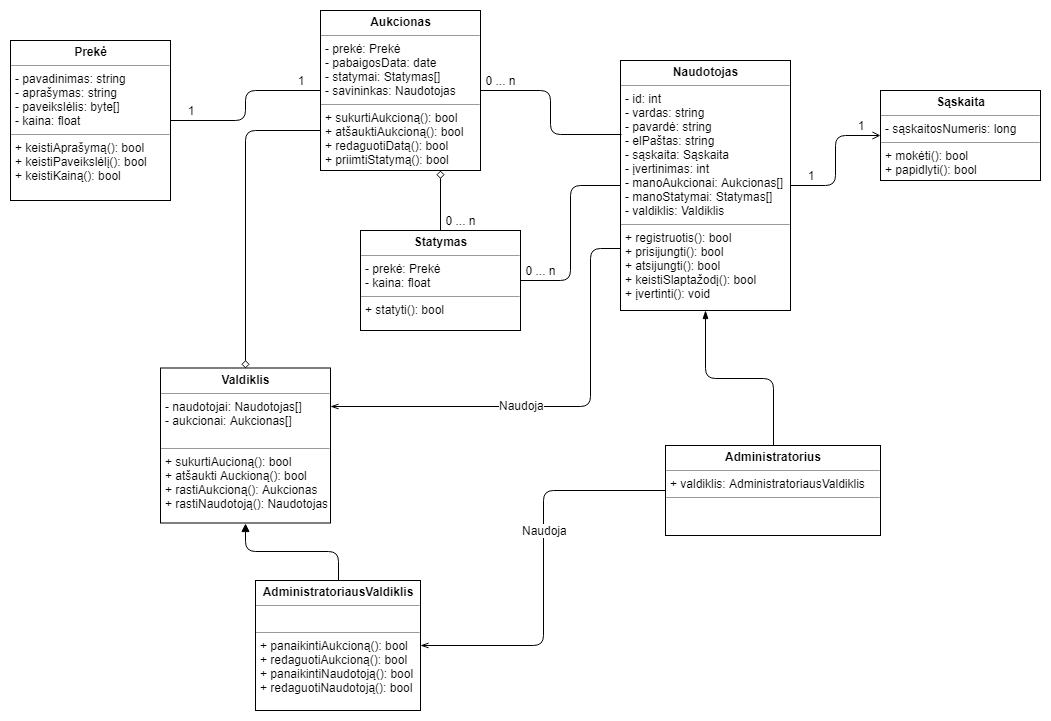
\includegraphics[width=\linewidth]{img/umlClassDiagram.png}
\label{fig:usecase}
\caption{Struktūrinis dalykinės srities modelis}
\end{figure}
\noindent
\textbf{Esybių sąrašas:} \\
1. Naudotojas - esybė, atsakinga už naudotojo duomenų saugojimą, jo valdymą\\
2. Administratorius - naudotojo funkcionalumą išplečianti esybė, suteikianti galimybę atlikti administratoriaus operacijas\\
3. Sąskaita - kiekvienam naudotojui priklausanti esybė, sauganti informaciją apie naudotojo sąskaitą bei atliekanti mokėjimo operacijas sistemoje\\
4. Valdiklis - esybė, atsakinga už visos aukciono sistemos valdymą bei duomenų saugojimą\\
5. Administratoriaus Valdiklis - išplėstinė valdiklio esybė, papildyta administratoriui reikalingu funkcionalumu\\
6. Aukcionas - esybė, atsakinga už aukciono informacijos saugojimą bei jo valdymą\\
7. Statymas - esybė, aprašanti bei sauganti informaciją apie atliktą statymą\\
8. Prekė - esybė, apibūdinanti bei sauganti informaciją apie aukcione parduodamą prekę\\

\newpage
\section{UŽDUOTYS}
Šioje dokumento dalyje yra pateikiamos sistemos atliekamos užduotys  (\ref{fig:usecase} pav.) Pateikiamas pagrindinis scenarijus ir alternatyvūs.\\
\begin{figure}[H]
\centering
\includegraphics[width=\linewidth]{img/UseCaseDiagram.png}
\label{fig:usecase}
\caption{Sistemoje atliekamos užduotys}
\end{figure}

\subsection{Naudotojo atliekamos užduotys}
Šiame skyrelyje išskiriamos visos sistemos naudotojo užduotys (\ref{fig:usercd} pav.), jas aprašant pateikiamas ne tik pagrindinis scenarijus, bet ir alternatyvūs. Taip pat atliekama robastiškumo analizė kiekvienai užduočiai.

\begin{figure}[H]
\centering
\includegraphics[width=\linewidth]{img/userusecased.png}
\label{fig:usercd}
\caption{Naudotojo atliekamos užduotys}
\end{figure}

\subsubsection{Užduotis - Registruotis}
Skyriuje pateikiamas užduoties registruotis aprašymas. Pateikiama užduoties robastiškumo analizės diagrama.\\
\textbf{Užduotis:}  Registruotis \\
\textbf{Scenarijus:} Naudotojas prisijungimo lange paspaudžia mygtuką registruotis. Sistema atidaro registracijos langą. Naudotojas suveda prisijungimo vardą, slaptažodį  \\
\textbf{Alternatyvūs scenarijai:} \\
\textbf{Nuoroda į reikalavimą: } 


\newpage

\sectionnonum{REZULTATAI}
Sistema išanalizuota taikant ICONIX metodą. Pateikti funkciniai ir nefunkciniai reikalavimai, apibrėžtas struktūrinis dalykinės srities modelis. Taip pat aprašytos sistemoje atliekamos užduotys, išanalizuoti pagrindiniai ir alternatyvūs užduočių scenarijai.
\newpage

\sectionnonum{PERŽIŪROS METU RASTOS KLAIDOS}
1. Perrašyti funkciniai reikalavimai.
\end{document}
